\documentclass [xcolor=svgnames, t] {beamer} 
\usepackage[utf8]{inputenc}
\usepackage{booktabs, comment} 
\usepackage[absolute, overlay]{textpos} 
\usepackage{pgfpages}
\usepackage[font=footnotesize]{caption}
\useoutertheme{infolines} 

\AtBeginSection[]{
  \begin{frame}
  \vfill
  \centering
  \begin{beamercolorbox}[sep=8pt,center,shadow=true,rounded=true]{title}
    \usebeamerfont{title}\insertsectionhead\par%
  \end{beamercolorbox}
  \vfill
  \end{frame}
}


%\definecolor{brownbrown}{RGB}{56, 28, 0}
%\definecolor{brownred}{RGB}{228, 0, 43}

%\setbeamercolor{title in head/foot}{bg=brownred, fg=brownbrown}
%\setbeamercolor{author in head/foot}{bg=myuniversity}
\setbeamertemplate{page number in head/foot}{}
\usepackage{csquotes}


\usepackage{amsmath}
\usepackage[makeroom]{cancel}
\usepackage[absolute,overlay]{textpos}

%\usepackage{textpos}

\usepackage{tikz}

\usepackage{media9} 

\usetheme{Madrid}
%\definecolor{myuniversity}{RGB}{56, 28, 0}
%\usecolortheme[named=myuniversity]{structure}
\usepackage{tikz}



\title[Viscosidad]{Clase No.6: Propiedades de los fluidos}
\subtitle{Ley de viscosidad de Newton, tipos de fluidos y tipos de flujo}
\institute[]{Departamento de Ingenier\'ia Civil y Agr\'icola\\ Facultad de Ingenier\'ia  \\Universidad Nacional de Colombia - Sede Bogot\'a}
\titlegraphic{
\includegraphics[height=2.0cm]{escudoUnal.png}}
\author[LAM]{Luis Alejandro Morales \\ \href{https://lamhydro.github.io}{https://lamhydro.github.io}}


%\institute[]{Department of Earth, Environmental, and Planetary Sciences  \\Brown University}
\date{\today}


\addtobeamertemplate{navigation symbols}{}{%
    \usebeamerfont{footline}%
    \usebeamercolor[fg]{footline}%
    \hspace{1em}%
    \insertframenumber/\inserttotalframenumber
}

\begin{document}
\begin{frame}
\maketitle
\end{frame}


%%%%%%%%%%%%%%%%%%%%%%%%%%%%
\logo{\vspace{-0.2cm}
\includegraphics[height=0.8cm]{escudoUnal.png}~%
}
%%%%%%%%%%%%%%%%%%%%%%%%%%



\begin{frame}
\frametitle{Table of Contents}
\tableofcontents
\end{frame}


\section{Ley de viscosidad de Newton}
\begin{frame}{Ley de viscosidad de Newton}
\vspace{-0.5cm}
\begin{columns}
\column{0.5\textwidth}
\begin{block}{Viscosidad}
La \textbf{viscosidad} es una medida de la resistencia de un fluido a fluir (resistencia al corte). Esta determina la tasa de deformaci\'on de un fluido que es generada cuando este es sometido a un esfuerzo cortante $\tau$. Por ejemplo es mucho mas f\'acil moverse en aire que en el agua, ya que esta ultima tiene una viscosidad 50 veces mas alta. Mucho mas dif\'icil es el movimiento en aceite que podr\'ia tener 300 veces mas viscosidad que el agua. 
\end{block}
\column{0.5\textwidth}
% Fig 2.23 Cengel 
\begin{figure}[h]
\centering
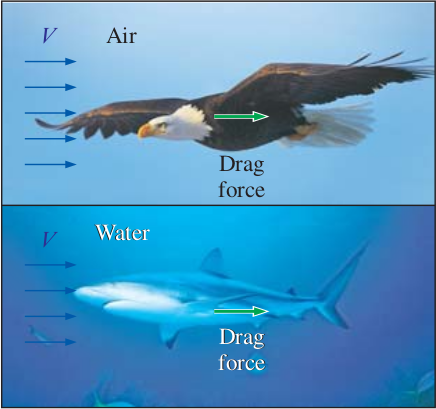
\includegraphics[width=0.9\textwidth]{visco0}
\caption{El fluido ejerce una fuerza de arrastre sobre el cuerpo en movimiento debido a la fricci\'on causada por la viscosidad.}
%\label{visco0}
\end{figure}
\end{columns}
\end{frame}


\begin{frame}{Ley de viscosidad de Newton}
Si consideramos un fluido que se mueve a una velocidad $u$ en un plano horizontal como resultado de una fuerza horizontal la cual produce un esfuerzo cortante, tenemos que el angulo de deformaci\'on $\delta \theta$ crece continuamente con el tiempo si $\tau$ se mantiene.

% Fig 1.6 White
\begin{figure}[h]
\centering
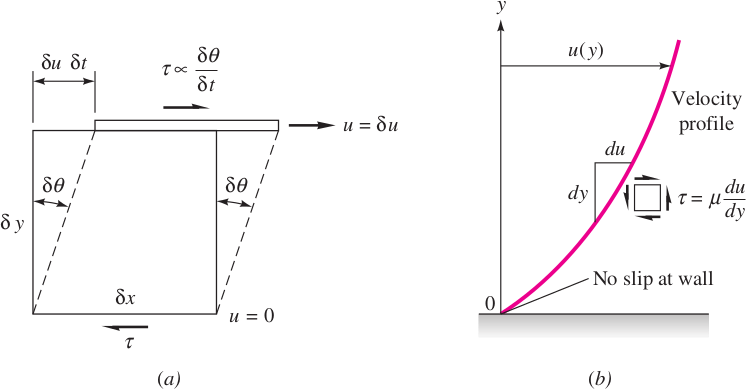
\includegraphics[width=7cm]{visco}
\caption{a)Deformaci\'on de un fluido que fluye sobre una superficie horizontal a velocidad $u$ y  b) perfil de velocidades de fluido en la capa l\'imite.}
%\label{visco}
\end{figure}

\end{frame}

\begin{frame}{Ley de viscosidad de Newton}
\vspace{-0.4cm}
% Fig 1.6 White
\begin{figure}[h]
\centering
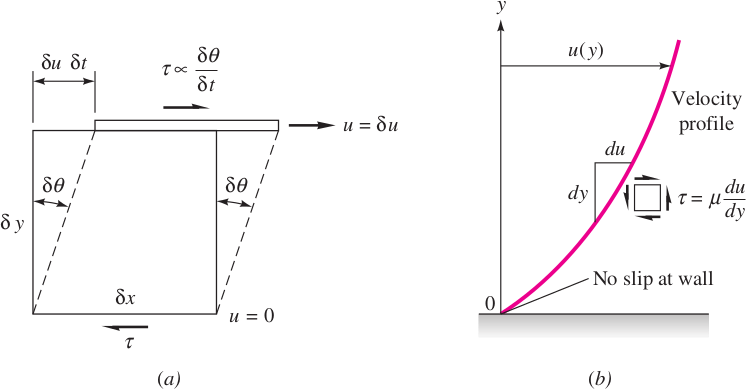
\includegraphics[width=7cm]{visco}
\caption{a)Deformaci\'on de un fluido que fluye sobre una superficie horizontal a velocidad $u$ y  b) perfil de velocidades de fluido en la capa l\'imite.}
%\label{visco}
\end{figure}

Por lo tanto, en fluidos como el agua, el aceite o el aire, la tasa de deformaci\'on se relaciona linealmente con el esfuerzo:
\begin{equation}
\tau \propto \frac{\delta \theta}{\delta t}
\label{vis1}
\end{equation}
\end{frame}

\begin{frame}{Ley de viscosidad de Newton}
\small
\vspace{-0.4cm}
% Fig 1.6 White
\begin{figure}[h]
\centering
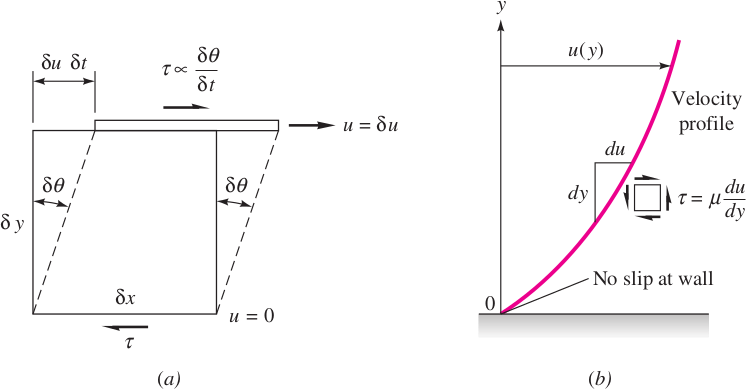
\includegraphics[width=6cm]{visco}
\caption{a)Deformaci\'on de un fluido que fluye sobre una superficie horizontal a velocidad $u$ y  b) perfil de velocidades de fluido en la capa l\'imite.}
%\label{visco}
\end{figure}
\vspace{-0.4cm}
De la figura~\ref{visco}a:
$$
\tan \delta \theta = \frac{\delta u \delta t}{\delta y}
$$
En el limite infinitesimal cuando $\delta \theta$ se hace pequen\~no, $\tan \delta \theta \approx \delta \theta$ y la ecuaci\'on anterior se convierte en:
$$
\frac{d\theta}{dt}=\frac{du}{dy}
$$
la cual expresa la equivalencia entre la tasa de deformaci\'on y el gradiente de velocidad.

\end{frame}

\begin{frame}{Ley de viscosidad de Newton}
\begin{block}{Ley de viscosidad de Newton}
Reemplazando en la ecuaci\'on~\ref{vis1} y teniendo en cuenta que la constante de proporcionalidad es el coeficiente de viscosidad $\mu$, conocido como viscosidad \emph{din\'amica} o \emph{absoluta}, tenemos:
\begin{equation}
\tau = \mu \frac{d \theta}{d t} = \mu \frac{d u}{d y}
\label{vis2}
\end{equation}
La ecuaci\'on~\ref{vis2} es conocida como la Ley de viscosidad de Newton y es validad exclusivamente para flujos laminares.
\end{block}
Si analizamos el perfil de velocidades en la \textbf{capa limite} la cual es la capa de fluido mas cercana a la placa solida inferior, la velocidad $u \approx 0$ y $\tau$ es m\'aximo en cercan\'ias a la placa solida. Dicho fen\'omeno es conocido como la \textbf{condici\'on de no deslizamiento} en fluidos viscosos. 

\end{frame}

\begin{frame}{Ley de viscosidad de Newton}
\begin{block}{Dimensiones de la viscosidad}
$\mu$ tiene dimensiones ${FT/L^2}$ o ${M/LT}$, en SI son $kg/m.s$, en BG son $slugs/ft.s$ y en CGS son $g/cm.s = 1\ poise$. 
\end{block}
\end{frame}

\begin{frame}{Placas paralelas}
\vspace{-0.4cm}
Un problema  cl\'asico es el flujo inducido entre una placa inferior fija y una placa superior que se mueve a una velocidad $\mathbf{V}$ (ver Figura~\ref{pla}). La distancia entre las placas es $h$ y dicho espacio esta ocupado por un fluido Newtoniano. Si las placas son grandes, el movimiento permanente induce una distribuci\'on de velocidad $u(y)$  (ver Figura~\ref{pla}) en donde $v=w=0$ y la aceleraci\'on es cero. De acuerdo con lo anterior, a un balance de fuerza sobre un elemento de fluido resulta en un esfuerzo constante en cualquier punto del fluido. Por tanto la Equaci\'on~\ref{vis2} se convierte en:

\begin{columns}
\column{0.6\textwidth}
% Fig 1.8 White
\begin{figure}[h]
\centering
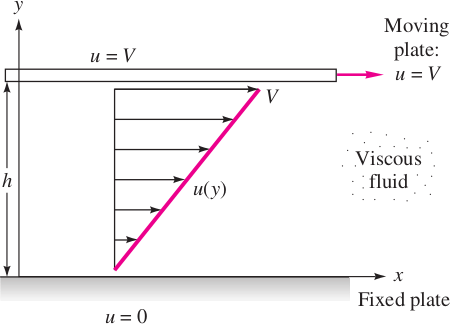
\includegraphics[width=5cm]{plate}
\caption{Flujo viscoso inducido por el movimiento relativo de dos placas paralelas.}
\label{pla}
\end{figure}

\column{0.4\textwidth}
$$
\frac{du}{dy}=\frac{\tau}{\mu}=\text{const}
$$
\end{columns}
\end{frame}

\begin{frame}{Placas paralelas}
Integrando esta ecuaci\'on para $u$, tenemos
$$
u=a+by
$$
lo cual indica una distribuci\'on lineal de la velocidad tal como se muestra en la Figura~\ref{pla} en donde $a$ y $b$ son constantes que se eval\'uan como:
$$
u= 
\begin{cases}
0 = a+b(0) & \quad \text{en}\ y=0 \\
V = a+b(h) & \quad \text{en}\ y=h 
\end{cases}
$$
de donde $a=0$ y $b=V/h$. Reemplazando en la ecuaci\'on, el perfil de velocidades entre las placas esta dato por:
\begin{equation}
u=V\frac{y}{h}
\label{upl}
\end{equation}
\end{frame}

\begin{frame}{Variaci\'on de la viscosidad con la temperatura}
\begin{block}{Efecto en gases}
Como la actividad molecular, la cual es la causa principal para la generaci\'on de esfuerzos de corte, se incrementa con el aumento de $T$, $\mu$ aumenta. Sin embargo, $\mu$ es independiente de la presi\'on. 
\end{block}
\begin{block}{Efecto en l\'iquidos}
Como la \emph{cohesi\'on} es la causa predominante de la viscosidad, cuando la $T$ incrementa, la cohesi\'on decrese y por tanto tambi\'en $\mu$ 
\end{block}
\end{frame}

%\begin{frame}{Variaci\'on de la viscosidad con la temperatura}
%La viscosidad es una propiedad termodin\'amica de los fluidos que depende de la presi\'on $p$ y de la temperatura $T$. Sin embargo, la variaci\'on de $\mu$ con respecto a la presi\'on es menor, mientras que la variaci\'on con respecto a la temperatura es significativa.
%La viscosidad de un gas incrementa con la temperatura. De acuerdo con esto existen dos leyes al respecto:
%\begin{equation}
%\frac{\mu}{\mu_0} \approx 
%\begin{cases}
%\left( \frac{T}{T_0} \right)^n & \quad \text{ley de potencia} \\
%\frac{(T/T_0 )^{3/2}(T_0 + S)}{T+S} & \quad \text{ley de Sutherland} 
%\end{cases}
%\label{vist}
%\end{equation}
%
%donde $\mu_0$ es la viscosidad a una temperatura absoluta $T_0$ (usualmente 273 K). Las constantes $n$ y $S$ son constantes ajustadas con base en datos. Por ejemplo para aire, $n\approx 0.7$ y $S\approx 110$ 
%\end{frame}
%
%\begin{frame}{Variaci\'on de la viscosidad con la temperatura}
%En l\'iquidos, la viscosidad decrece con la temperatura de una forma casi exponencial $\mu \approx ae^{-bT}$. Con base en esta ecuaci\'on esta expresi\'on es derivada:
%\begin{equation}
%\ln \frac{\mu}{\mu_0} \approx  a + b \left(\frac{T_0}{T}\right)+ c\left(\frac{T_0}{T}\right)^2
%\label{visf}
%\end{equation}
%
%en donde para agua con $T_0 = 273.16\ K$ y $\mu = 0.001792\ kg/(m.s)$, $a=-1.94$, $b=-4.80$ y $c=6.74$ con una  exactitud del $\pm 1$ \%.
%\end{frame}


\section{Tipos de fluidos}
\begin{frame}{Tipos de fluidos}
%\begin{columns}
%\column{0.5\textwidth}
%\begin{textblock*}{6cm}(0.4cm,3cm) % {block width} (coords)
\begin{block}{Tipos de fluidos}
\begin{itemize}
\item Fluidos Newtonianos
\item Fluidos no Newtonianos
\begin{itemize}
%\item Fluido ideal
\item Fluido pl\'astico
\item Fluido seudopl\'astico
\item Fluido dilatable
\end{itemize}
\end{itemize}
\end{block}
%\end{textblock*}
%\column{0.5\textwidth}
%\begin{textblock*}{6.5cm}(6.8cm,3.3cm) % {block width} (coords)
%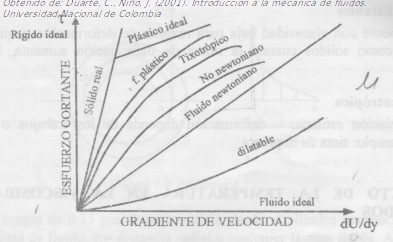
\includegraphics[width=0.9\textwidth]{tflui}
%\end{textblock*}
%\end{columns}
\end{frame}

\begin{frame}{Tipos de fluidos}
\vspace{-0.5cm}
\begin{block}{Fluidos Newtonianos}

Son fluidos que se comportan de acuerdo con la siguiente ecuaci\'on:
$$
\tau = \mu \frac{d u}{d y}
$$
en donde la pendiente de la recta determina la viscosidad $\mu$.
\end{block}
\begin{textblock*}{4.6cm}(3.4cm,4.5cm) % {block width} (coords)
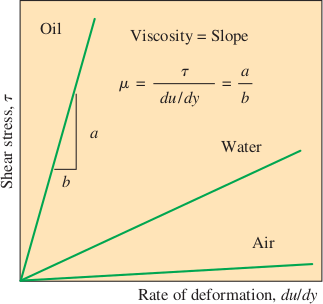
\includegraphics[width=\textwidth]{fnewt}
\end{textblock*}
\end{frame}

\begin{frame}{Tipos de fluidos}
\begin{textblock*}{6.5cm}(0.4cm,2.5cm) % {block width} (coords)
$\mu$  = 0.01 $P$\\
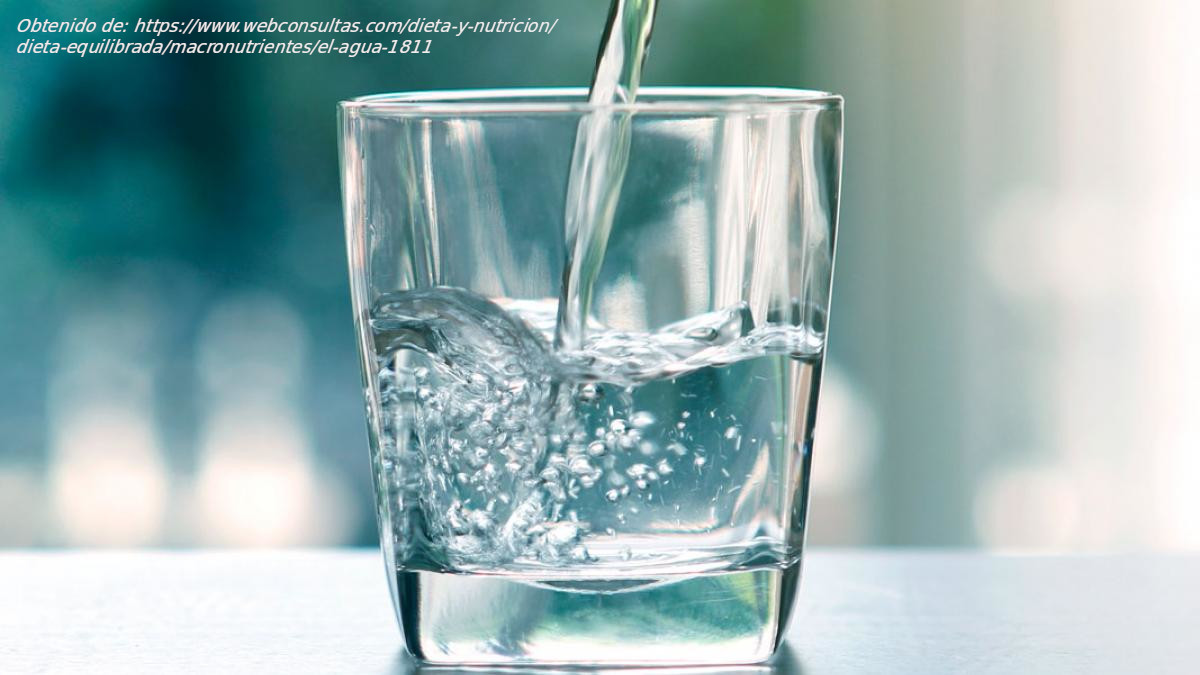
\includegraphics[width=0.9\textwidth]{fnew}
\end{textblock*}
\begin{textblock*}{6.5cm}(6.8cm,2.5cm) % {block width} (coords)
$\mu$  = 0.006 $P$\\
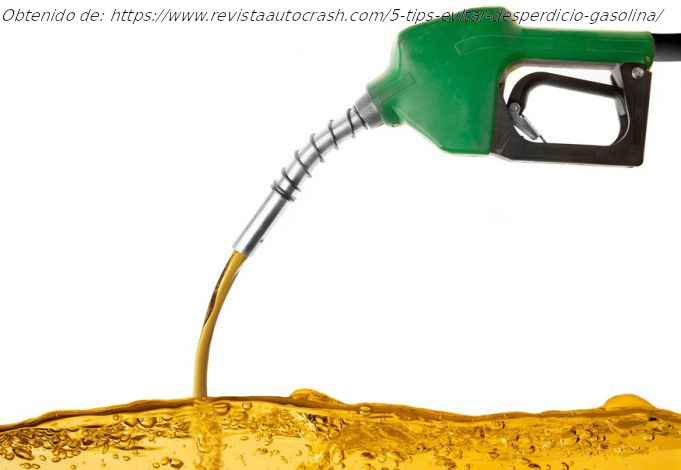
\includegraphics[width=0.9\textwidth]{fnew2}
\end{textblock*}
\end{frame}

\begin{frame}{Tipos de fluidos}
\begin{block}{Fluidos no Newtonianos}
Se deforman de manera que la tensi\'on de corte no es proporcional al gradiente de velocidades por lo que $\mu$ es variable. La deformaci\'on de estos fluidos  puede clasificarse como pl\'astica.
%Fluidos que no siguen la ecuaci\'on lineal ~\ref{vis2} son llamados \textbf{no Newtonianos}. Mientras que en los flujos Newtonianos la viscosidad es constante con el aumento del esfuerzo, en los fluidos no Newtonianos la viscosidad cambia. Algunos tipos de fluidos no Newtonianos son:
\end{block}
\begin{textblock*}{5cm}(4.0cm,4cm) % {block width} (coords)
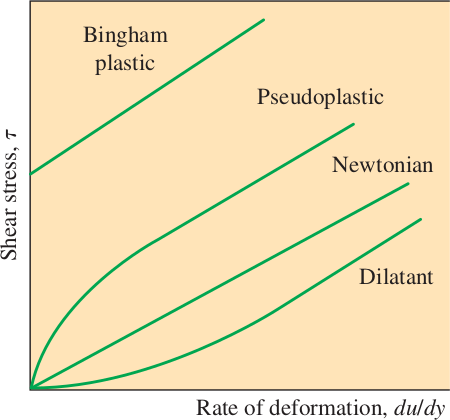
\includegraphics[width=\textwidth]{nonew}
\end{textblock*}
\end{frame}

\begin{frame}{Tipos de fluidos} 
\begin{block}{Fluidos no Newtonianos} 
\begin{itemize}
%\item \textbf{Ideal}: La resistencia al esfuerzo de corte es nula ya que se asume que $\mu$ =0. Los fluidos ideales no existen, pero pueden ser \'utiles en an\'alisis te\'oricos.
\item \textbf{Pl\'astico}: Requieren un esfuerzo inicial antes de que inicie a fluir o deformarse. Por ejemplo: mayonesa, crema de dientes, lodos, salsa de tomate. La salsa de tomate no sale del recipiente a menos que se le aplique un esfuerzo inicial (se sacuda o se exprima el recipiente). 
\item \textbf{Seudoplastico}: La resistencia disminuye a altas tasas de deformaci\'on. Por ejemplo: pintura y soluciones de pol\'imeros. La pintura es gruesa antes de aplicarla pero se hace delgada cuando se aplica a una alta taza de deformaci\'on.
\item \textbf{Dilatante}: Incrementa su resistencia cuando la tasa de deformaci\'on incrementa. Fluyen f\'acilmente con viscosidad baja para razones de deformaci\'on peque\~nas. Ejemplo: arena movediza. 
%\item \textbf{Tixotr\`opico}: La relaci\'on esfuerzo - deformaci\'on depende de los trabajos o deformaciones anteriores. Cuanta más presión se someta el fluido a esfuerzos de corte, más disminuye su viscosidad.
\end{itemize}
\end{block}
\end{frame}

\begin{frame}{Tipos de fluidos}
\begin{textblock*}{4cm}(0.4cm,2cm) % {block width} (coords)
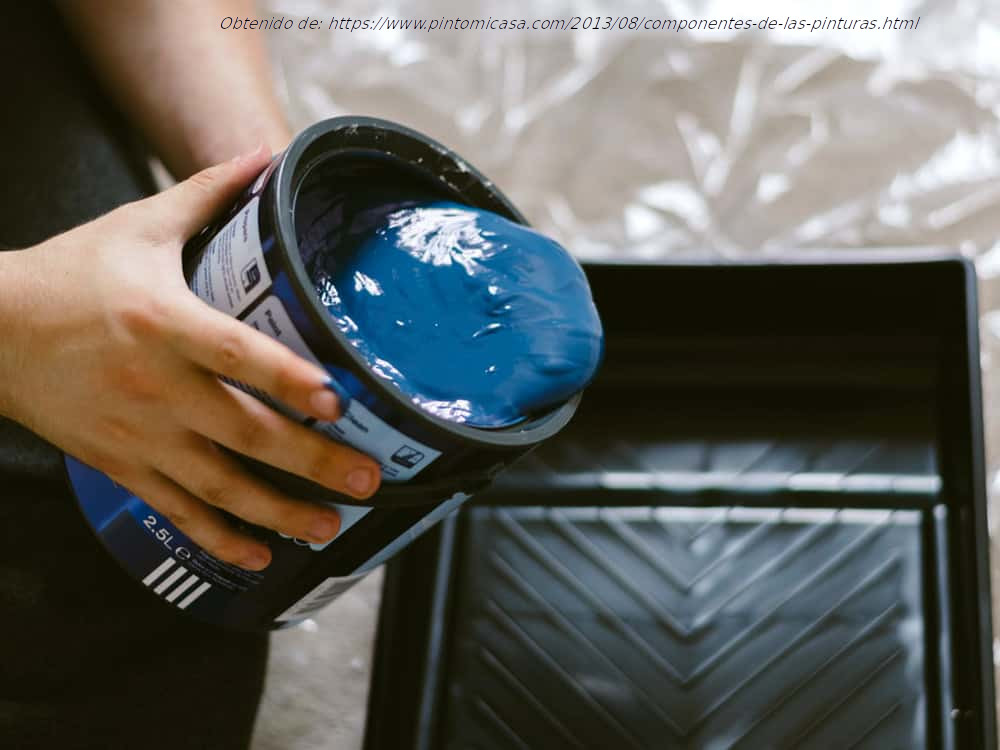
\includegraphics[width=\textwidth]{fnonew}
\end{textblock*}
\begin{textblock*}{4cm}(4.5cm,2cm) % {block width} (coords)
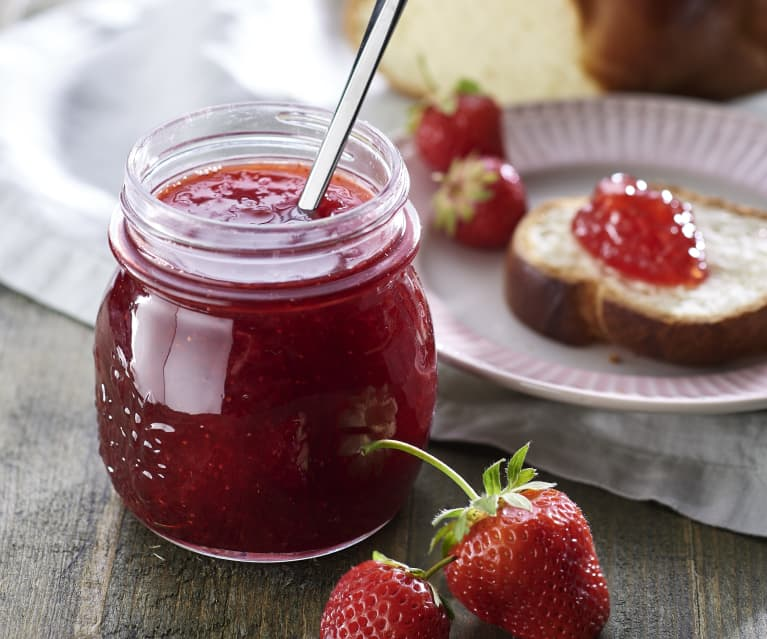
\includegraphics[width=\textwidth]{fnonew3}
\end{textblock*}
\begin{textblock*}{4cm}(8.6cm,2cm) % {block width} (coords)
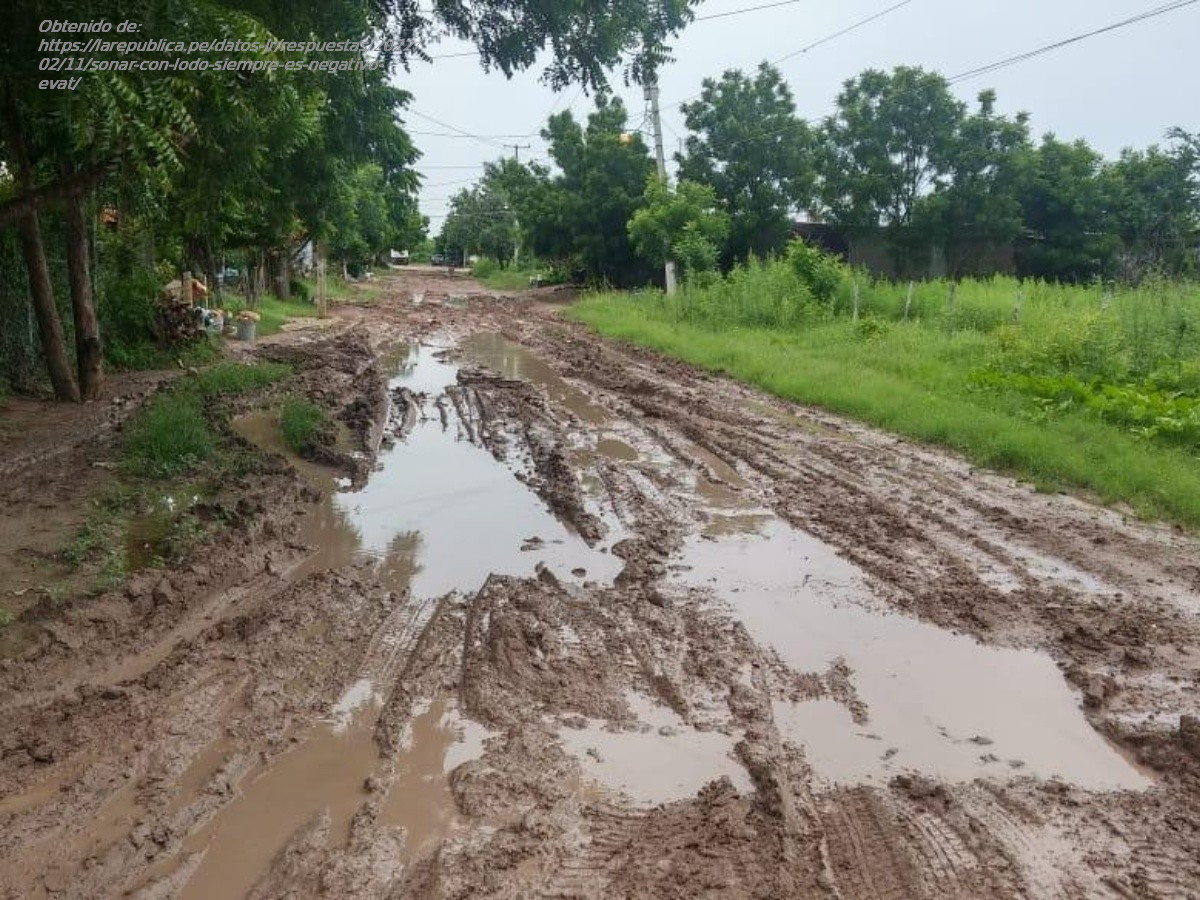
\includegraphics[width=\textwidth]{fnonew4}
\end{textblock*}
% Fig 2.26 Cengel
%\begin{figure}[h]
%\centering
%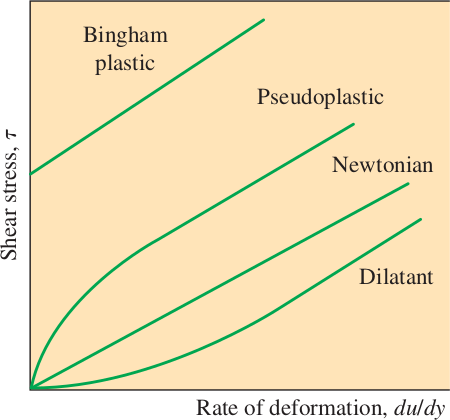
\includegraphics[width=8cm]{nonew}
%\caption{Variaci\'on del esfuerzo con la tasa de deformaci\'on para fluidos Newtonianos y no Newtonianos.}
%\label{nonew}
%\end{figure}
\end{frame}

\section{Tipos de flujo}

\begin{frame}{Tipos de flujo}
\vspace{-0.3cm}
\begin{block}{Flujo laminar}
\begin{center}
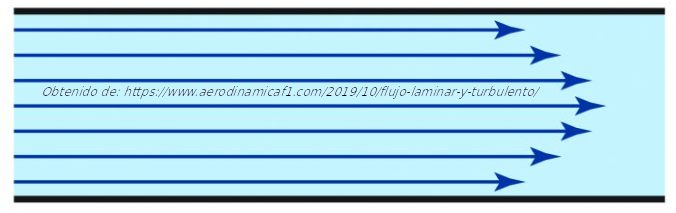
\includegraphics[width=0.5\textwidth]{flami}
\end{center}
Es un fluido que fluye puramente en l\'aminas o capas en donde las part\'iculas se mueven paralelamente gracias a la viscosidad del fluido. Este flujo esta gobernado por la \emph{Ley de viscosidad de Newton}.
\end{block}
\begin{columns}
\column{0.5\textwidth}
\begin{textblock*}{6cm}(0.4cm,5.9cm) % {block width} (coords)
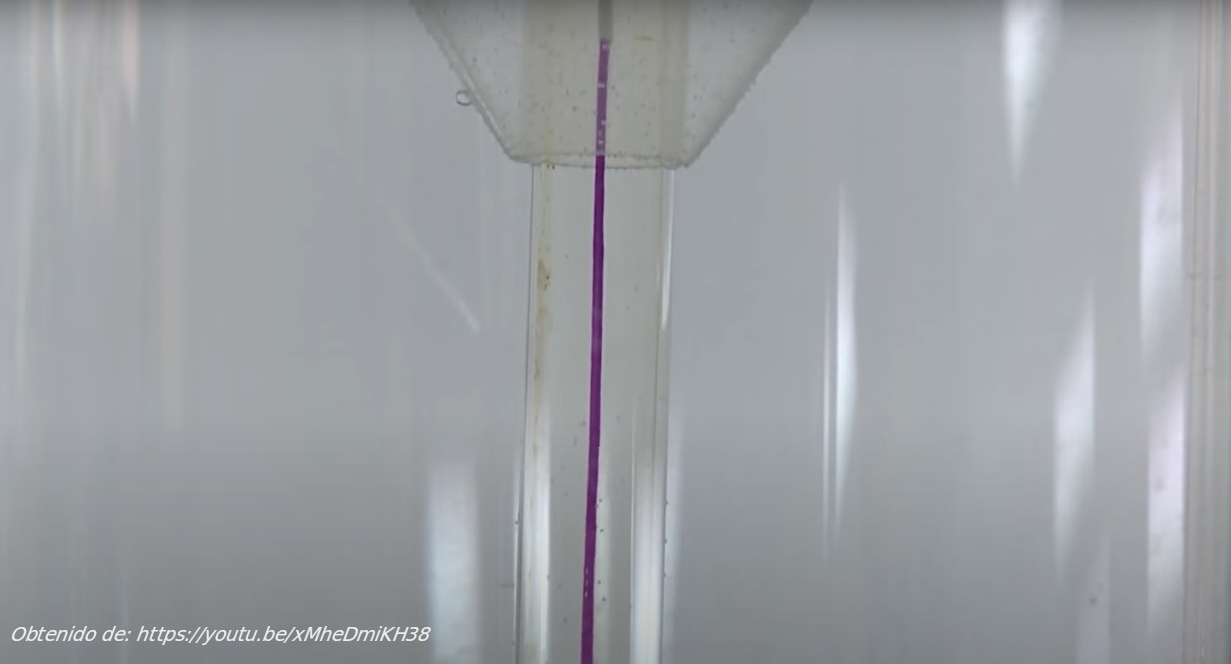
\includegraphics[width=\textwidth]{flami2}
\end{textblock*}
\column{0.5\textwidth}
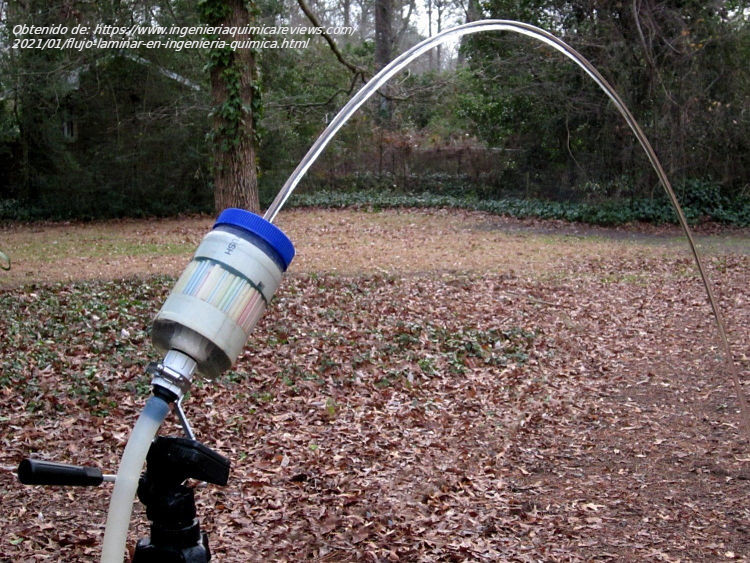
\includegraphics[width=\textwidth]{flami3}
\end{columns}
\end{frame}

\begin{frame}{Tipos de flujo}
\vspace{-0.3cm}
\begin{block}{Flujo turbulento}
\begin{center}
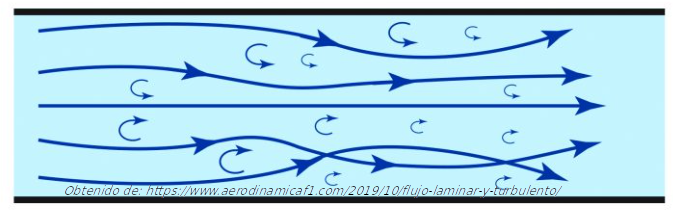
\includegraphics[width=0.5\textwidth]{ftur}
\end{center}
En flujo turbulento, las part\'iculas se mueven en forma desordenada y ca\'otica. Este flujo es el mas frequente en problemas de ingenier\'ia como por ejemplo el flujo en tuber\'ias, en rios, y en estructuras hidr\'aulicas. El esfuerzo de corte en flujo turbulento se puede expresar como:
$$
\tau = (\mu + \nu)\frac{du}{dy}
$$
donde $\nu$ es un factor que depende de la densidad del flujo y de las caracter\'isticas del movimiento (efecto de la turbulencia).
\end{block}
\end{frame}

\begin{frame}{Tipos de flujo}
\vspace{-0.3cm}
\centering
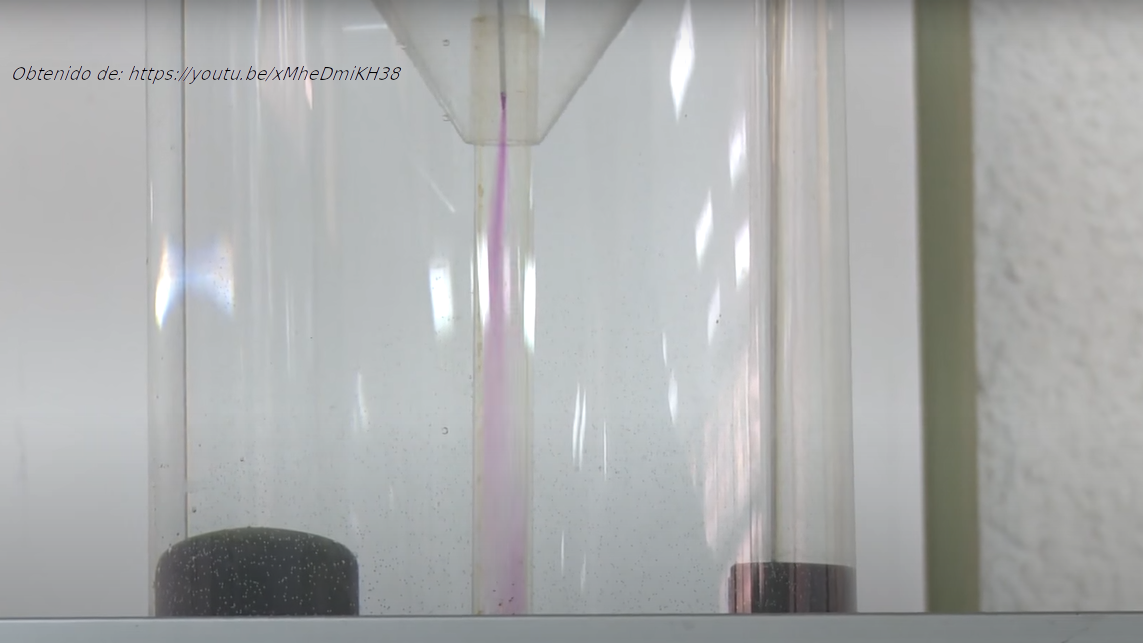
\includegraphics[width=0.55\textwidth]{ftur2}
\begin{columns}
\column{0.5\textwidth}
\begin{textblock*}{4.0cm}(0.4cm,4.7cm) % {block width} (coords)
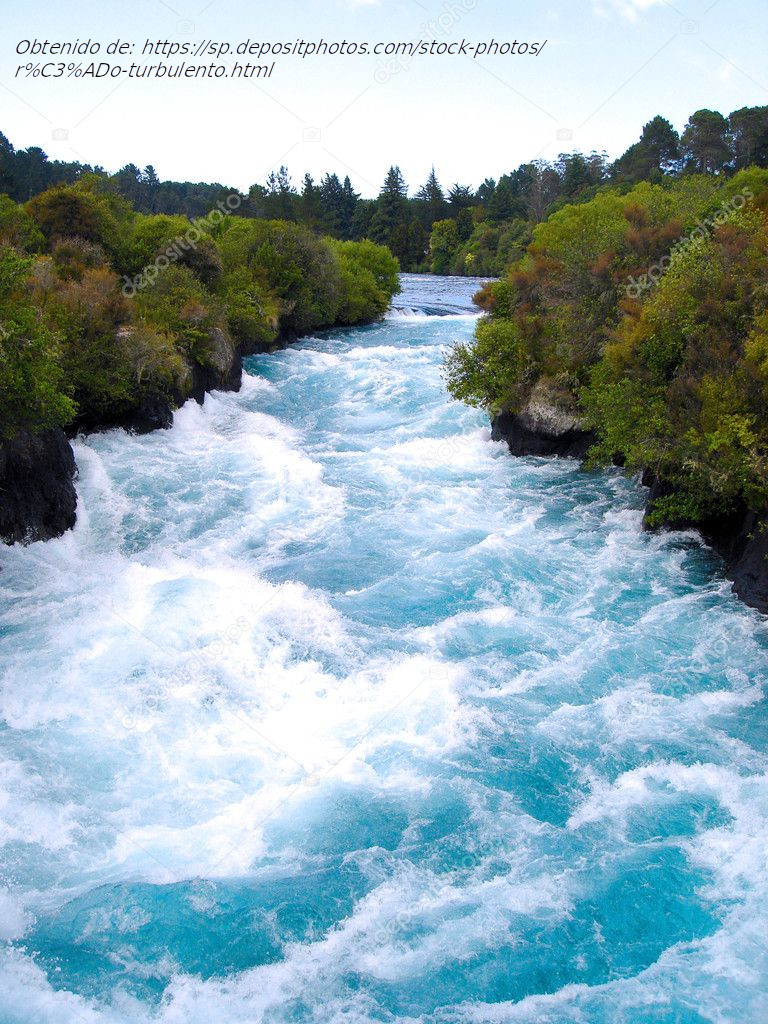
\includegraphics[width=\textwidth]{ftur3}
\end{textblock*}
\column{0.5\textwidth}
\begin{textblock*}{6cm}(6.5cm,4.7cm) % {block width} (coords)
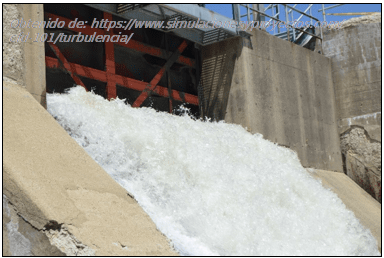
\includegraphics[width=\textwidth]{ftur4}
\end{textblock*}
\end{columns}
\end{frame}


\begin{frame}{Tipos de flujo}
\begin{block}{El Numero de Reynolds}
El numero de Reynolds $Re$ es un numero adimensional que caracteriza el movimiento de un fluido y se define como:
\begin{equation}
Re=\frac{\rho VL}{\mu}=\frac{VL}{\nu}
\label{re1}
\end{equation}
donde $V$ es la velocidad, $L$ es la longitud caracter\'istica del flujo y $\nu=\mu/\rho$  es la \textbf{viscosidad cinem\'atica}. La ecuaci\'on~\ref{re1} indica que $Re$ es la relaci\'on de las fuerzas convect\'ivas o inerciales y las fuerzas viscosas presentes en el fluido. De acuerdo con esto, $Re$ muy bajos significan flujos muy viscosos donde las fuerzas inerciales son despreciables. $Re$ moderados son flujos \textbf{laminares} que se mueven suavemente en capas paralelas. Un $Re$ alto es caracter\'istico de un flujo \textbf{turbulento}.  
\end{block}
\end{frame}

\section{Resumen}
\begin{frame}{Resumen}
\footnotesize
\begin{block}{Ley de viscosidad de Newton}
$$
\tau = \mu \frac{du}{dy}
$$
donde $\mu$ es la viscosidad din\'amica o absoluta y $u$ es la velocidad del fluido.
\end{block}
\begin{block}{Tipos de fluido}
\begin{itemize}
\item \textbf{Newtoniados}: $$\mu = \frac{\tau}{du/dy} =\ Cte $$
\item \textbf{No Newtoniados}: $$\mu = \frac{\tau}{du/dy} \ne\ Cte $$
\end{itemize}
\end{block}
\begin{block}{Tipos de flujo}
\begin{itemize}
\item \textbf{Laminar}: Fluye en laminas o capas y sigue la ley de viscosidad de Newton. $NR$ bajos.
\item \textbf{Turbulento}: Fluye en forma ca\'otica. $NR$ altos.
\end{itemize}
\end{block}
\end{frame}



\end{document}

